%\documentclass[prb,preprint]{revtex4} 
\documentclass[twocolumn,preprintnumbers,amsmath,amssymb,aps,prx]{revtex4}
% The line above defines the type of LaTeX document.
% Note that AJP uses the same style as Phys. Rev. B (prb).

% The % character begins a comment, which continues to the end of the line.
\usepackage{amsmath}  % needed for \tfrac, \bmatrix, etc.
\usepackage{amsfonts} % needed for bold Greek, Fraktur, and blackboard bold
\usepackage{graphicx} % needed for figures
\usepackage{pythontex}

\begin{document}

% Be sure to use the \title, \author, \affiliation, and \abstract macros
% to format your title page.  Don't use lower-level macros to  manually
% adjust the fonts and centering.

\title{Molecular dynamics simulation of synchronization in driven particles}
% In a long title you can use \\ to force a line break at a certain location.

\author{Tiare Guerrero}
\email{guer9330@pacificu.edu} % optional
%\altaffiliation[permanent address: ]{101 Main Street, 
%  Anytown, USA} % optional second address
% If there were a second author at the same address, we would put another 
% \author{} statement here.  Don't combine multiple authors in a single
% \author statement.
%\affiliation{Department of Physics, Pacific University, Forest Grove, OR 97116}
% Please provide a full mailing address here.

\author{Danielle McDermott}
\email{mcdermott@pacific.edu}
\affiliation{Department of Physics, Pacific University, Forest Grove, OR 97116}

% See the REVTeX documentation for more examples of author and affiliation lists.
\date{\today}

\begin{abstract}
  Synchronization
  plays a key role in many physical processes.
  We discuss a simple
  numerical model %that
  of synchronized particles 
  %exhibits
  %provides insight
  %to synchronization behavior
  %and
  %atoms on surfaces.
  %voltage driven superconducting vortices
  %confined in a Josephson junction,
  %and ac and dc driven
  %charge and spin density waves.
  %We present the basics
  using
  molecular dynamics simulations
  for particles moving through
  a viscous liquid.
  %Simplified models
  %such as 
  %What problem did you study and why is it important?
  Modeling synchronization
  with simulations and table-top experiments
  can 
  provide insight
  to complex behaviors
  in the natural world.
  We drive 
  particles
  across a washboard potential energy landscape, 
  a 
  common 
  technique to isolate complex 
  synchronized patterns 
  in both simulations and experiments.
  %as observed in 
  %experiments %al systems 
  %of %interest to condensed matter physics %including 
  %magnetically driven colloidal particles
  %confined by light-fields.
  %exhibit a variety of synchronization effects.
  %in
  %  Numerical model
  %
  %applied to single and multiple particle systems.
  %so we model the dynamics of each particle
  %with 
  %overdamped equations of motion.
  Our results show a variety of synchronization effects 
  in single particle systems, 
  %and detect synchronization using
  %measurements of
  which we characterize by 
  plotting 
  particle velocity as a function of applied driving force 
  and phase diagrams of position versus velocity.
  %We demonstrate how to 
  %visualize
  %the system with
  %numerical representations of the landscape
  %and
  %animations of the particle motion.
  %We include sample code
  %and exercises for students
  %with 
  %opportunities
  %to reproduce our results and propose
  %new numerical experiments.
  %With only a few particles in two-dimensions,
  %the simulation runs quickly,
  %making this an appropriate model for undergraduates to explore.  
\end{abstract}
% AJP requires an abstract for all regular article submissions.
% Abstracts are optional for submissions to the "Notes and Discussions" section.

\maketitle % title page is now complete

\section{Introduction} %
%
%Outline
%------------------------------------------------------------------
%synchronization = widest audience possible
Synchronization is a universal phenomena
in which
individual oscillators change frequency due
to external stimuli \cite{Pikovsky2003}.
The
flickering patterns of
candle flames mediated by temperature fluctuations \cite{Okamoto2016},
vibrations of singing wineglasses interacting 
through sound waves \cite{Arane2009}, 
and metronomes vibrating through a supporting platform \cite{Jia2015}
are examples of in-phase coupled oscillations. %of components 
Biological systems benefit from cooperative
synchronization -- %such as 
birds coordinate wing flaps
to optimize energy use during flight \cite{Portugal2014},
frogs alternate croaking patterns \cite{Aihara2014},
humans clap in time with music \cite{Tranchant2016}
and 
at a cellular level, 
neurons simultaneously fire in cardiac muscle \cite{MartinHall1999}
and brain tissue \cite{Singer1999}.
External forcing can cause or regulate 
synchronization %. % is often achieved via external forcing
%such as when
%single particle oscillators
-- %For instance,
an electrical pacemaker %(an electrical generator)
regulates a heart beat 
and 
a pulsed light modifies the
flashing pattern of fireflies .% \cite{Agrawal2013}.

%Christiaan Huygens 
%[has been adapted into many useful technologies...]
Synchronized phase-locking or mode-locking 
first appeared in the scientific literature
with 
Huygens' 1665 experiments on
motions of synchronized 
pendula in wall-mounted clocks \cite{Bennett2002}.
%Even when started out of phase, 
%Huygens demonstrated the tendency of
%coupled pendula tend to swing in time
%due to interactions through the wall 
%phase locking
A locked-mode is an integer frequency ratio.
In Huygens clocks,
%even when started out of phase, 
the pendula were observed swing at same rate -- a 1:1 mode.
For simple pendula of different lengths,
a 2:1 mode can be seen when a pendulum four
times the length of another swings with twice the period.
%
%to a mode or frequency ratio  
%of an integer number \cite{Bak1986}.
%Dynamical mode locking
%The phenomena

%\section{Colloidal Models}
%\label{sec:colloids}

Complex dynamics can be studied with
colloid particles in experiments or simulations.
Typical colloids are   
plastic spheres suspended in
de-ionized water or silica beads suspended in organic solvent.
%experimental - colloids specifically
Because 
colloids are large %-- a few microns in size
and move slowly %-- a few microns per second,
particle position 
can be imaged in real time 
with an optical camera \cite{Pertsinidis2001}. %(see Table ~\ref{tab:1}).
Experimental measurements of 
step-by-step dynamics of 
colloids performing phase-locked motions
are useful for
understanding synchronization at a single particle level \cite{Juniper2015}.
 
%due to the large size and slow speed of the particles.
%Individual colloids exhibit 
%Brownian motion,
%where particles change direction %in a seemingly random fashion
%due to 
%collisions 
%with unseen particles comprising the suspending fluid \cite{}.
%[elaborate - move to associated problems?].

Light is a
tool for manipulating the colloidal environment.
A circular optical trap uses 
radiation pressure from 
a laser beam to confine colloids \cite{Ashkin1997}.
%Since photon density is high at the beam center,
A colloid centered in the beam is %subject to a
uniformly bombarded by photons while 
%form a circular pattern with a higher density 
%central 
%energy minimum.
%optical trap  trap colloids
%with radiation pressure  which uses  photon 
%control colloid motions 
%A  is designed
off-center colloids %away from center
collide with photons unevenly,
creating a net force.
%Colloids at a trap edge
%experience a net force
%due to the 
Depending on the %shape of the trap and
location of the particle in the trap,
the radiation pressure either moves colloids toward the beam center 
%local minimum 
or ejects it from the trap.
An optically trapped colloid executing Brownian motion
is a useful probe of microscopic forces ~\cite{Volpe2013}.
%In experiments
Diffraction gratings can be used to create
more complex light environments, 
%with one or more laser beams,
such as periodic patterns of minima
suitable for synchronization studies \cite{Grier2003}.

A single particle oscillator
in a potential well is 
like a skateboarder in a half-pipe or
a child on a swing.
%If subject to an applied force,
 How a particle moves
 in an optical landscape can
 change
 when 
 subject to external driving forces.
 %Individual particles can
 %move with synchronized location and velocity
 % with the environment
 %motions
 %that lock together particle .
 A confined oscillator may 
 synchronize its location
 to the periodic pattern of the external drive,
 moving back and forth in time with
 the beat. 
 %The relationship between the driving force and
 %landscape can change the pattern of motion.  
 With a constant or 
 dc drive the landscape modulates 
 the particle velocity, below some threshold  
 the dc force is not strong enough to push the particle
 across a potential maximum so the average velocity is zero,
 a phenomena referred to as pinning \cite{Reichhardt2017}.
 Above the pinning threshold,
 a particle subject to a constant
 drive force will increase its speed at a rate propotional
 to the external drive.  
 %and dissipating energy from the system at all driving forces.
 A sinusoidal or ac drive can create mode-locking,
 where the average particle velocity
 is fixed for a range of dc drive forces \cite{Reichhardt2015}.
 %This synchronization phenomena
 %is useful for understanding the complex dynamical 
 %systems.  
 
%Numerical modeling of colloids can provide mechanistic insight
%that can be difficult to achieve in experimental conditions
%where Brownian motion and other sources of noise dominate.
%external forces
%The
%dynamics of particles subject to 
%an applied external force apply to many physical systems.
%For instance the flow of charges in a conductor,
%or cells responding to a chemical gradient.
%The external force 
%increases the diversity of dynamical behaviors,
%and can cause particles to flow in
%a variety of non-linear complex patterns
%that may be 
%synchronized.
%Disordered chaotic dynamics are also possible,
%where irregular, unpredictable time evolution of
%nonlinear systems occurs in mechanical oscillators \cite{chaos}.
%-------------------------------------------------------------

%Given the prevalence of synchronization,
%it is the subject of many computational models.
Here we perform numerical studies 
on the synchronized dynamics
of confined particles driven over
a washboard shaped potential energy landscape.
%Numerical studies %of harmonic systems
%can yield insights
%to the mechanics of naturally oscillating systems.
We chose this model for its
relevance to condensed matter systems
and ease of simulation.
%---------------------------------------------------------------
%kinks and nanofriction
%-----------------------------------------------------------------
%transition from synchronized to chaotic
%describe types of physical systems - particle types
%%In this work,
%we perform 
%numerical simulations of confined, driven particles
%to model a variety of physical phenomena.
%-----------------------------------------------------------------------
%paper outline
%In the following paper
%In Section~\ref{sec:colloids} we describe colloid particles,
%an relevant
%experimental analog of our simulations.
We describe
our molecular dynamics model for a single particle in Section~\ref{sec:MD}.
%In this section, we restrict our discussion to a single particle,
%and include additional information
%for multiple particles in Section~\ref{sec:sync}.
%including various  and confining environments.
We summarize
our results 
%in Section~\ref{sec:results} 
including synchronized motion of a single confined particle
driven across a periodic landscape in 
Section~\ref{sec:one}.
%In Section~\ref{sec:sync}
%we 
%extend the model to include multiple particles,
%and show how confined 
%interacting particles respond to the same applied driving force.
%including stationary propagation of high density kinks
%in Sec.~\ref{sec:kink}.
%We include code to simulate
%and visualize the landscape and dynamics in this section
%and supplementary material.
%we
%demonstrate how uniform environments and applied forces
%and create synchronized flow patterns.
%We present these results using standard tools of non-linear oscillators
%such phase diagrams of velocity versus position.
%PHASE DIAGRAMS SHOWING COUPLING, OR QUASI-PERIODIC COUPLING
%INDICATE COOPERATIVE MOTION IN THE Q1D SUBSTRATE
%In Section~\ref{sec:quasiperiod},
%we show how an aperiodic landscape modifies the particle dynamics.
%Finally we explore the transition to chaotic dynamics in 
%Section~\ref{sec:chaos}
%and conclude 
We include 
exercises for interested students 
in Section~\ref{sec:problems}.
In Section~\ref{sec:conclusion}
we describe how our results apply 
to physical systems
such as dusty plasmas, superconducting vortices and Josephson junctions.




%Here we model the microscopic dynamics of phase locking in a colloidal model system using molecular dynamics (MD).

\section{Molecular Dynamics Simulation}
\label{sec:MD}

We use a classical model for 
studying the dynamics of $N$ interacting particles,
using the net force on each particle to calculate
its trajectory.
Particles are confined in a two-dimensional (2D) 
simulation of area $A = L \times L$ where $L=36.5 a_0$
where $a_0$ is a dimensionless unit of length.
An individual particle $i$ has
position $\vec{r}_i = x_i \hat{x} + y_i \hat{y}$
and velocity $\vec{v}_i = d\vec{r}_i/dt$.
The edges of the system are treated with
periodic boundary conditions
such that a particle leaving the edge of the system is mapped
back to a position within the simulation boundaries 
by the transformation $x_i+L \rightarrow x_i$ and $y_i+L \rightarrow y_i$.
%and particles interact across PBC.
We show a schematic of the system in Fig.~\ref{fig:landscape0}(a).

We confine the particles using a position dependent 
potential energy function, called a landscape or substrate.
 %The landscape potential energy $U(\vec{r})$ is static 
 %with fixed minima and maxima
 %that are periodic or quasi-periodic,
 %as described in Sec.~\ref{sec:results}.
% 
The landscape is modulated in the y-direction
with the periodic function 
%% %that used in Sec.~\ref{sec:one}
% where 
 \begin{equation}
   U(y) = U_0 \cos{(N_p \pi y / L)}
     \label{eq:ysubstrate}
\end{equation}
 where $N_p$ are the number of periods,
 % $L$ is the period length,
 and $U_0$ is an adjustable parameter
 to set the depth of the minima
 with simulation units of energy $E_0 = 1$. 
 %We define the substrate strength to be
 %the maximum force the substrate can exert on a particle 
 %
 We plot this function in 
 Fig.~\ref{fig:landscape0}
 for $N_p = 3$. %to illustrate the features of
 In Fig.~\ref{fig:landscape0}(a) we show 
 the $x-y$ plane with a contour plot of $U(y)$ %Eq.~\ref{eq:ysubstrate}
 to illustrate
 the 2D potential energy landscape,
 where 
 the maxima are colored red and the minima colored blue.
 The confining force on a particle $i$
 %arises from a potential function 
 %creating a landscape of potential minima and maxima
 %that modify the force on a particle as a function of position
 is calculated as 
 $\vec{F}^{l}_i(\vec{r}_i) = -\nabla U_l(\vec{r}_i)$.
 In Fig.~\ref{fig:landscape0}(b) we plot the function
 $U(y)$ to illustrate how the magnitude
 $\vec{F}^{l}_i$ is calculated from particle position $y_i$.  
 %in the $y-$direction.

 
 Particles are subject an external time-dependent driving force
$\vec{F}_{D}(t)$
applied parallel to the y-direction.
We model this force as
\begin{equation}
  \vec{F}^{d}(t) = [F^{dc} + F^{ac} \sin(\omega t)] \hat{y},
    \label{eq:drive}
\end{equation}
with modifiable parameters including
a constant component $F^{dc}$,
and a time dependent component with amplitude $F^{ac}$
and frequency $\omega = 2 \pi f$.
%in the positive $y-$direction.
%but it may 
%be zero or negative depending the the parameters and time.
%%%%%%%%%%%%%%%%%%%%%%%%%%%%%%%%%%%%%%%%%%%%%%%%%%%%%%%%%%%%%%%%%%
%RAMP!!!
%%%When $F^{dc}$ is non-zero,  we slowly increase $F^{dc}$ from zero to avoid transient behavior by ensuring the particle is subject to a smoothly varying force. We illustrate the increase of $F^{dc}$ in Fig.~\ref{fig:0}(a).
%%%%%%%%%%%%%%%%%%%%%%%%%%%%%%%%%%%%%%%%%%%%%%%%%%%%%%%%%%%%%%%%

%because
The inertia of 
small particles is reduced by interactions
with fluid particles \cite{Purcell1977}.
In our model
we assume 
colloids are overdamped
-- i.e. colloids are suspended in a continuous viscous fluid
that dissipates energy %at a rate
such 
that the particles do not accelerate.
%that greatly impedes their motions.
Energy dissipation from the fluid is modeled
with a frictional force on particle with velocity $\vec{v}_i$ as
%that removes energy from
%the particles,
%which we model as
$\vec{F}^{drag}_i = -\eta \vec{v}_i$
%proportional to the particle velocity 
with a friction coefficient $\eta$
proportional to the fluid viscosity.
We discuss friction models for
spheres moving through fluids in 
%Section~\ref{sec:problems}
Exercise~\ref{ex:reynolds}. %for more information
%We model the particle dynamics  with an overdamped equation of motion. Models with inertia set to zero are appropriate for moving through a high viscosity fluid
\begin{center}
\begin{figure}[h!]
\centering
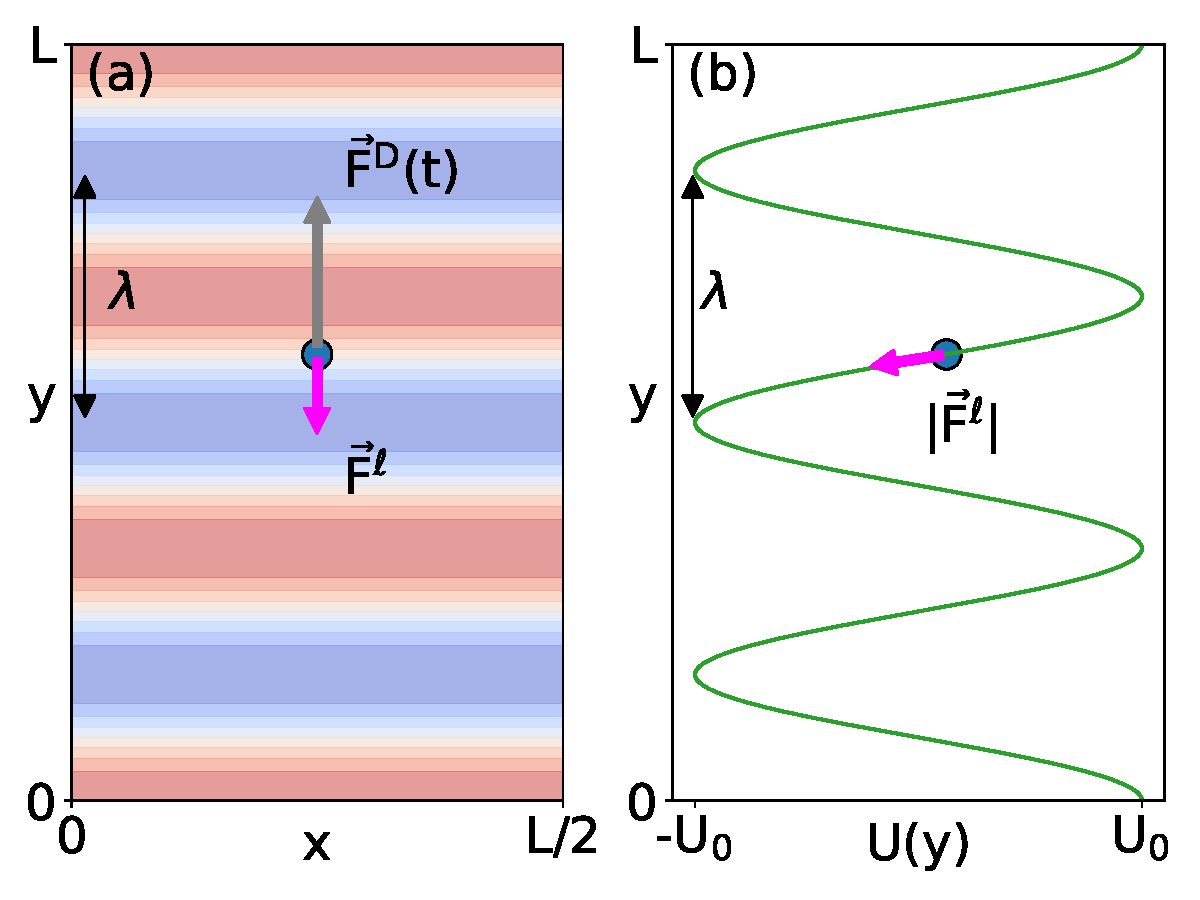
\includegraphics[width=\columnwidth]{landscape.pdf}
\caption{
  Schematic of the simulation
  of a single particle
  driven across a washboard potential
  energy landscape.
  The period of the landscape is $\lambda = L/N_p$,  
  %is marked in red,
  where $N_p = 3$.  
  The force due to the landscape %$\vec{F}^l$
  is calculated from the gradient of the potential
  energy 
  $\vec{F}^l = -\nabla U(\vec{r})$.
  (a) View of the $x-y$ plane. %of the simulation
  The time-dependent applied driving force $\vec{F}^d$
  is parallel to the y-axis.
  The landscape is shown with a contour plot,
  with maxima in the potential energy marked in red
  and minima marked in blue.
  A particle is shown in the region between minima and maxima
  subject to competing forces of the landscape and applied driving force.
  (b) The potential energy function
  along the y-axis $U_l(y)$.  
  The particle in (a) is shown at the same $y-$position.
  The slope of $U_l(y)$ is the 
  magnitude of force $\vec{F}^l$. %is calculated
  %as the slope of this function,
  %directed along the $y-$direction in panel (a).
  }
\label{fig:landscape0}
\end{figure}
\end{center}
Newton's second law for an individual particle
%$m \vec{a}_i = \sum \vec{F}$
is simplified
by the assumption $\vec{a}_i$ is zero. % in the overdamped model.
%Newton's second law can be rearranged %for the velocity
%to
The overdamped equation of motion for an isolated particle is
%solved for velocity 
\begin{equation}
  \eta \vec{v}_i = \vec{F}^l_{i}(\vec{r}_i) + \vec{F}^{d}(t).
    \label{eq:motion}
\end{equation}
with  $\eta = 1$ in units of $v_0 / F_0$. 
%(see Table~\ref{tab:1}).
%and Exercise~\ref{ex:reynolds}.
%In %Section~\ref{sec:problems}
%Exercise~\ref{ex:n2l}
%we invite the reader to confirm this result.
The equation of motion provides a direct calculation of the velocity
of an individual particle from its location $\vec{r}_i$ %in the simulation
and the simulation time.

The molecular dynamics simulation is controlled by a $for()$ loop
which runs from an initial to maximum integer number of time steps.
%$t_i$.
Each integer time step interval %$t_{i+1}-t_i$
represents a simulation time of $\Delta t$ 
simulation units $\tau$.  %as described in Table 1
At each time step
we evaluate the net force on each particle as a function of its position
$\vec{r}_i(t)$
and then integrate
the equation of motion to move particles
to an updated position.
%$\vec{r}_i(t+\Delta t)$.%
Since the acceleration as zero,
the integration of the equation of motion
is performed via 
the Euler method 
\begin{equation}
  \vec{r}_i(t+\Delta t) = \vec{v}_i(t) \Delta t + \vec{r}_i(t)
    \label{eq:euler}
\end{equation}
for a small time step $\Delta t = 0.001 \tau$.
In %Section~\ref{sec:problems}
Exercise~\ref{ex:euler}
we describe 
the numerical methods for 
solving differential equations.
%
The units of the simulated variables are summarized in Table ~\ref{tab:1}.

\begin{table}[h!]
\centering
\caption{Simulation parameters and units and comparable
  experimental values~\cite{Juniper2015}.
  Blanks %in the experimental parameters
  indicate
  units, rather than parameters that
  are not easily represented by a single value.}
%{\it might be more appropriate to match Juniper parameters more precisely given our focus...}}
\begin{ruledtabular}
\begin{tabular}{c c c } %p{5cm}}
Quantity & Simulation Unit & Experimental value\\
\hline
length &  $a_0 = 1$ & $ a_0 \sim 1.5 \mu m$\\
energy & $E_0 = 1$ & \\ %$ < E_0 <$ \\
%electric potential & $V(r_{ij}) = E_0/r_{ij}$ \\
%energy & $E_0 = q^2{Z^*}^2/4\pi \epsilon \epsilon_0 a_0$ \\
%dimensionless interaction strength & $q$ \\
%effective colloidal charge & $Z^*$ \\
%solvent dielectric constant & $\epsilon \epsilon_0$\\
force & $F_0 = E_0 / a_0$ & \\ %$<F_0<$\\
time &  $ \tau = \eta a_0 / F_0 $ \\ %& $ < \tau <$\\
velocity &  $ a_0 / \tau $ &  $v \sim 5 \mu m/s $\\
driving period & $T = 100 \tau$ & $T \sim 1.3$ s \\
viscosity coefficient & $\eta = F_0 \tau / a_0 $ & $\eta \sim 10^{-3}$ Pa-s \\
%juniper uses water–ethanol mixture
substrate period & $\lambda = 1.825 a_0$ & $\lambda = 3.5 \mu m$ \\
substrate amplitude & $U_0 = 0.058 E_0$ & $U_0 = 75 k_B T \sim 2 J$ \\
temperature & $T_0 = 0$ \footnote{to learn more about the effects
  of temperature on this simulation
  see Ex.~\ref{ex:brownian} where we study the limit
  $U_0 \sim k_B T$.} & $T \sim 300K $ \\

%FROM JUNIPER2015
%l¼3.5 mm and a laser power per trap of WE0.75mW (trap stiffness: k=3.8\times10^7 kg /s^2; trap depth: V0 = 75 k_B T
%ref51
%Juniper, M. P. N., Besseling, R., Aarts, D. G. A. L. & Dullens, R. P. A. Acousto- optically generated potential energy landscapes: potential mapping using colloids under flow. Opt. Express 27, 28707–28716 (2012).
%U(x) measured in ratio of k_BT from -75 to -25
%0 < vAC < 8 micrometer/s and frequency f=0.25 to 0.75 Hz.
%0 < vDC < 5 micrometer/s
%convert to force units?
%check when steps exist - in Juniper - steps don't exist for n=1or n=3, even though steps exist for n¼0,2,4,5 and 6.
%flexible chains
%dipole interaction $\Gamma \propto B^2$
%\Gamma =15 (B=0.43mT) and a stiff chain at \Gamma=392 (B=2.2mT).
%Kink
%16 particles in a strong potential energy landscape of 15 minima (trap spacing: l¼5.5 mm; laser power per trap: WE1.75 mW; trap stiffness: k¼8.7?10?7 kg s?2; trap depth: V0¼200 kBT),

%Volpe AJP Parameters
%We will consider a silica microparticle in water with radius R=1micro m, mass m=11picograms, viscosity eta=0.001 Ns/m^2; $\gamma=6\pi \eta R$,  T=300K, and \tau=0.6\micro s.
%thermofisher off the shelf paramagnetic beads
%https://www.thermofisher.com/us/en/home/references/protocols/proteins-expression-isolation-and-analysis/protein-isolation-protocol/m-270-carboxylic-acid.html
%~2\times10^9 beads per 30 mg -> 1.5 \times 10^-11 g, 15 ng

\end{tabular}
\end{ruledtabular}
\label{tab:1}
\end{table}

%\section{Results}
%\label{sec:results}
% We demonstrate how a single particle (Sec.~\ref{sec:one})
% and many particles
% move (Sec.~\ref{sec:sync})
% in response to this applied force in a variety of environments.
% In Sec.~\ref{sec:kink} we set $F^{dc}$
% to zero and track the motion
% of a high density area of a particle chain
% (i.e. kink dynamics).
 %The driving force does add energy into the system, and some of it is lost.
%
\section{Mode-locking of a single particle}
% In subsection headings, only the first word is capitalized.
\label{sec:one}

A single particle %on this landscape
responds to the applied driving force
by moving across the landscape %maxima
synchronized with 
the period of $F^d(t)$.
%applied driving force.
%along the y-direction
%({\it redundant, just refer back to eq. in Model?})
%and $V_{0y}=0.2$.
%This is illustrated in Fig.~\ref{fig:1}(a) where
%the red (blue) regions show local maxima (minima).
%
The numerical implementation of the landscape 
is calculated with Eq.~\ref{eq:ysubstrate} as 
\begin{equation}
  \label{eq:force}
  F^l_y(y) = -A_{p} \sin{(N_p \pi y / L)} 
\end{equation}
where the force is scaled with parameter $A_{p} = N_p \pi U_0/L$.
In this section, we fix the landscape parameters
to $A_{p} = 0.1$ force units
with $N_p=20$ minima %in the landscape
corresponding to a spatial period $\lambda = 1.825 a_0$.

%In Fig.~\ref{fig:0} 
The driven particle adjusts
its motion to traverse
the periodic landscape with the same rhythm as 
the applied time-dependent force $F^d(t)$.
When $F^d(t) > A_p$, a particle can 
overcome the barrier height of the landscape,
and 
the particle hops between minima in the energy landscape.
%
In Fig.~\ref{fig:0}(a)
we plot $F^d(t)$ %defined in Eq.~\ref{eq:drive}.
as a function of time with
%The time independent
constants $F^{dc}=0.1$, 
$F^{ac}=0.05$ and $f=0.01$ cycles per time unit $\tau$.
The temporal period of the driving force is
$T = 1/f = 100 \tau$.
%%%%%%%%%%%%%%%%%%%%%%%%%%%%
%RAMP
%To avoid transient oscillations at early times, the dc driving force is initially zero and slowly increased %$F^{dc}$. at a rate of $\Delta F^{dc} = 0.01$ every $\Delta t = 4$ time units  to the constant value $F^{dc}=0.1$. In Fig.~\ref{fig:0}(a) we plot $F^{dc}$ in blue to show the increase in  $F^{dc}$ for the first $40$ time units In orange we show  the combined ac and dc drive $F^d(t)$ when the magnitude of the ac applied force is initially zero.
%%%%%%%%%%%%%%%%%%%%%%%%%%%%%%%
%since $\sin{(0)}=0$.
We mark the maxima of $F^{ac}(t)$
with the
vertical dashed lines %in panels (a) and (b)
-- i.e. $\sin{(\omega t)} = 1$.
%
%
%with the initial driving force at is minimum value 
%$F^d(0) = F^{dc}$. 
%
In Fig.~\ref{fig:0}(b) 
we show the $y-$position of the particle
as a function of time.
We 
normalize $y$ by $\lambda$ %, the spatial period of the potential
to show  particle motion between substrate minima.  
The initial particle position is $y = 0 $. %1 a_0$,
%where the $F^l$ is negative.
%JUST BECAUSE
%causing the particle to move to
%a landscape minima at the start of the simulation.
As the driving force increases,
%the effects of the landscape become less obvious,
the motion of the particle
synchronizes with the driving period $T$.
We measure 
average particle velocity $\langle{v}_y\rangle$
as the average displacement %$\Delta y = y(t_0+T) - y(t_0)$
over the period of the driving force.
The particle moves
in the positive y-direction
through $\Delta y = 2 \lambda$ over the time period $T$,
with 
the average velocity 
$\langle {v}_y \rangle= 2 \lambda f$. % where $T = 1/f$.
The horizontal dashed lines
coincide with the condition the particle is at a substrate minima
where substrate force  $F^l = -A_p$,  
i.e. $\sin{(\pi y / \lambda)} = 1$.
%or $\pi y / \lambda = m \pi/2$, where $m = 1, 5, 7$, {\it etc.}
%Once the particle motion
%coincides with the applied drive,
%indicating synchronization,
The particle synchronizes its motion such that the 
driving force is maximum when the landscape 
force is minimum,
as indicated %with the coincidence of 
with the intersection of
vertical and horizontal lines.  
%i.e. the particle position $y/\lambda$.  
The slope of $y/\lambda$
is proportional to the net force on the particle.
This can be seen in 
Fig.~\ref{fig:0} %we demonstrate this relationship,
where local extrema appear in $y/\lambda$
when $F_{D}(t) \approx 0 $. 


\begin{center}
\begin{figure}[h!]
\centering
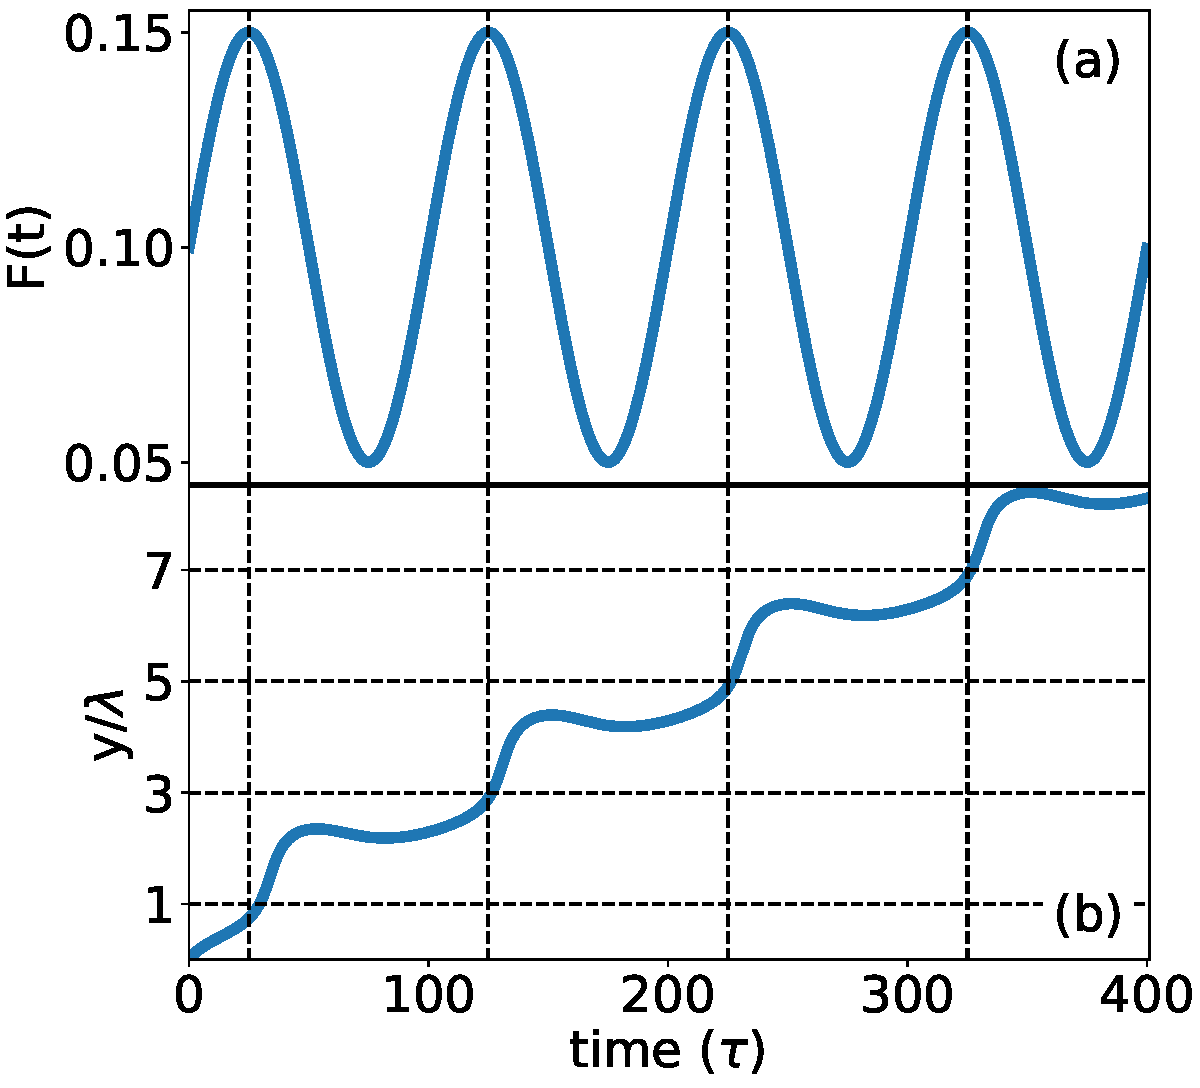
\includegraphics[width=\columnwidth]{single_particle.pdf}
\caption{(a) The applied driving force $F^d(t)$. % (Eq.~\ref{eq:drive}).
  %where the parameter $F^{dc}$ (blue) is slowly increased from zero %to a constant value %as described in the text.
  (b) 
  The $y-$position of the driven particle
  %of a single driven particle
  normalized by the period of the substrate $\lambda$.
  %as a function of time
  }
\label{fig:0}
\end{figure}
\end{center}

The competition between the driving force and landscape potential
can produce a variety of hopping patterns in the particle motion. 
%In Fig.~\ref{fig:0}
%reaching a minimum position
%of $y/\lambda = 1$
%over the total period $T = 100$.
%In Fig. ~\ref{fig:0}
%the average displacement during one time period is a single wavelength
%of the substrate $y(t_0+T) - y(t_0) = \lambda$.
%single dc case with figure
%dc_current 0.01
%ac_current 0.05
%ac_frequency 0.01
%fp_y 0.1
%
The relative values of $F^{ac}$, $F^{dc}$ and $A_p$
control the rate and distance a  particle moves 
forward and backward in the landscape.
To explore the possible hopping patterns,
we sweep through a range of $F^{dc}$ for fixed $F^{ac}$ and $A_p$
to illustrate
distinct oscillation modes. % as a function of $F^{dc}$.
A mode is a periodic pattern of hops
with a constant average particle velocity, $\langle {v}_{y} \rangle$
over a range of driving forces $F^{dc}$.
%as shown
In Fig.~\ref{fig:1} 
we keep $F^{dc}$ constant
for $10^5$ simulation timesteps
and 
measure the average velocity $\langle v_y \rangle $ 
as a function of $F^{dc}$,
with $F^{ac} = 0.05$, $f=0.01$, and the landscape %force $\vec{F}^{l}$
shown in Fig.~\ref{fig:0}.
%We plot the results in Fig.~\ref{fig:1} for 
The modes appear as 
discrete steps in $\langle v_y \rangle$ %occur because
across a range of $F^{dc}$,

%the average velocity of the particle
%is constant 
%despite the overall magnitude
%of $F^{dc}$.
Each step represents a different pattern of hops
between substrate minima
performed by the particle
due to the landscape confinement.  
In Fig.~\ref{fig:1} at %this occurs at 
low $F^{dc}$ the average velocity $\langle v_y \rangle$ is zero.
Since 
$A_p$ is large compared to the extrema of $F^{d}(t)$,
the particle oscillates back and forth
in a single minima with no net velocity.
At higher $F^{dc}$ the particle velocity 
$\langle v_{y} \rangle$ increases in steps of uniform height,
$\langle v_{y} \rangle = n \lambda f$,
where $n$ is an integer.
The step width is non-linear 
and can have a variety of
interesting patterns
such as a devil's staircase related to chaotic dynamics \cite{Bak1986}.
We note the individual steps
are not strictly horizontal 
since particles move continuously
through the landscape, so changes in $F^{dc}$
will create linear changes in 
net particle displacement that are observable
within a single step.

%$\lambda = L/N_p = 36.5/20 = 1.825$ is the spatial period, or wavelength
%of the landscape,
%and $f = 0.01$ cycles per time unit.

%This synchronization
%of the particle velocity can be measured
%in terms of the landscape period.
%Phase locked steps occur for average displacements integer
%multiples of the substrate period $n\lambda$.

We explore a range of parameters in Ex.~\ref{ex:parameters}
where 
we perform this sweep for several values
of $F^{ac}$ including the limiting case that the applied force
is a constant value.
When $F^{ac} = 0$, no steps appear
in the $\langle v_y \rangle $ vs $F^{dc}$ curve. 
When $F^{dc} - F^{ac} < -A_p$ the particle
moves in the negative y-direction 
during part of the cycle.
%We examine
The period of the substrate
can be used to control the
intrinsic velocity of the dc driven particle,
and the applied ac drive can cause mode-locking
which appears as non-linear 
steps in the force-velocity relationship.

In the following section
we include exercises to explore our numerical model,
including the 
to linear drag equation in Ex.~\ref{ex:reynolds}, 
the equation of motion in Ex.~\ref{ex:n2l},
and 
numerical integration techniques in Ex.~\ref{ex:euler}.
An extended model that includes finite temperature effects
is in Ex.~\ref{ex:brownian}.
We explore changes in the particle motion
with parameter changes in Ex.~\ref{ex:parameters}.
Methods to visualize the dynamics of the particle motion
are in Ex.~\ref{ex:animation}.


\begin{center}
\begin{figure}[h!]
\centering
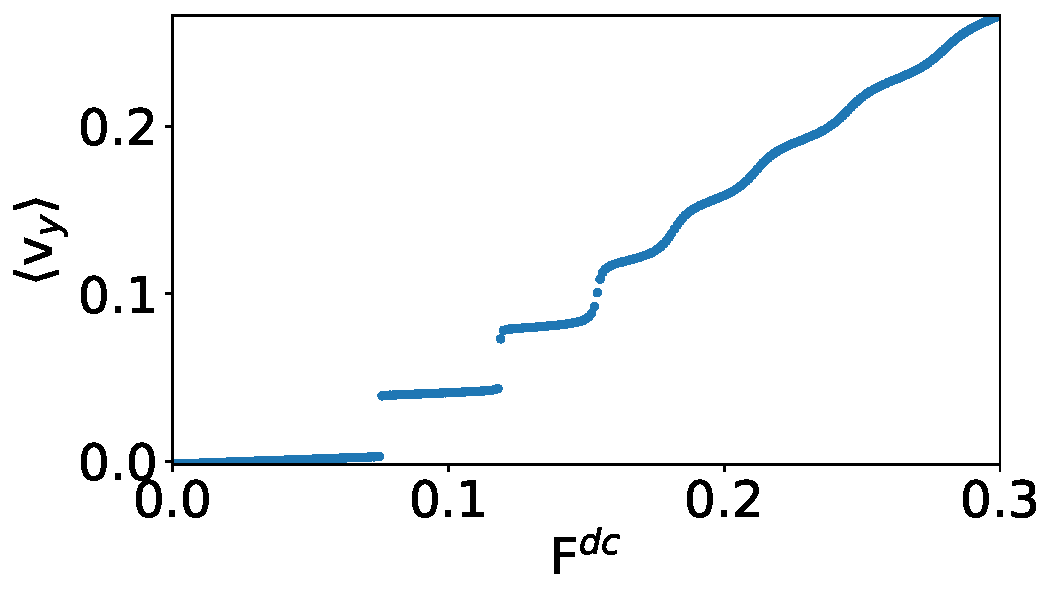
\includegraphics[width=\columnwidth]{sweep_FDC_vs_vx.pdf}
\caption{Average particle velocity  $\langle v_{y} \rangle$ as a function of $F^{dc}$,
  the constant parameter of $F^d(t)$ defined in Eq.~\ref{eq:drive}.
  The remaining parameters in $F^d(t)$ are as in Fig.~\ref{fig:0}, $F^{ac}=0.05$ and $f = 0.01$.  }
\label{fig:1}
\end{figure}
\end{center}

%In the animation available in Ref.~\cite{supp1} the magenta dot represents the average velocity of the particle $\langle v_{y} \rangle$ at which the particle in Fig. 1(a) is moving.

\section{Associated problems}
\label{sec:problems}	% You can label sections for reference

%\begin{enumerate}
%\item
\subsection{Drag Models and Reynolds Numbers.}
  Stokes' law describes the viscous drag on a sphere
  moving at velocity $\vec{v}$ as 
  $\vec{F}^{lin} = -3 \pi \eta D \vec{v}$ 
  where $\eta$ is the dynamic fluid viscosity and 
  $D$ is the particle diameter \cite{Taylor2005}.
  In simulation we
  subsume the constants $3 \pi D$
  such that $3 \pi D \eta \rightarrow \eta $.
  %
  Often drag forces are
  modeled as a polynomial series ~\cite{Taylor2005}
  \begin{equation}
    \vec{F}^{drag} = -b \vec{v} - c v^2 \hat{v} + \ldots  .
  \end{equation}
  %This model should be familiar to readers
  %of a standard classical mechanics text, such as Ref.
  %when studying 
  %models Millikan's oil drops.
  Truncating the series to the first term
  is justified by demonstrating the sphere
  has a low Reynolds number  
  $R = D v \rho / \eta$
  where $\rho$ is the fluid density and $v$ the particle's speed.
  When $R$ is small, the quadratic and higher order terms
  may be ignored in favor of the linear drag term.

  {\bf Using reasonable values for the
  experimental analog of this system, 
  show that the Reynolds number is small.}
  In addition to the values listed in Table ~\ref{tab:1}, 
 % Approximate experimental values for
 % a colloid size and speed
 % are $D = 1 \mu m$ and $v \sim 1 \mu m /s$.
 % %Likewise
 % To first order the viscosity is $\eta \sim 10^{-3}$ Pa-s 
 % since 
 % viscosity of water decreases with temperature
 % from $1.3 \times 10^{-3}$ Pa-s at $10^{\circ}$ C to 
 % from $0.31 \times 10^{-3}$ Pa-s at $90^{\circ}$ C,
 % where 1 Pascal is $1$ N/m$^2$.
  %Likewise
  the liquid density $\rho$ varies with temperature
  with $\rho \sim 10^3$ kg/cm$^3$ a reasonable
  first order approximation
  \cite{asce}.
  

%  [{\it could certainly do more with this question to make it more computational.  For instance, plot $R$ as a function of any of the parameters $v$, $D$ and $\rho$, include a temperature dependent $\eta(T)$ in the Brownian system.  Suggest students model something big to imagine their own life at low Reynolds number... fairly off topic...}]

\label{ex:reynolds}

%\item
\subsection{Equation of Motion}
  \label{ex:n2l}
  
  Newton's second law states that
  the acceleration of a particle $i$
  is proportional to 
  the sum of forces on the particle 
  \begin{equation}
  m_i \vec{a}_i = \sum \vec{F}_i
  \label{eq:n2l}
  \end{equation}
  where the constant of proportionality is the
  inertial mass $m_i$.  
  The addition of a dissipative force to a dynamical equation 
  of colloid motion 
  is typically modeled
  with a drag force proportional to the particle's velocity
  in the opposite direction of motion 
  $\vec{F}^{drag} = - \gamma \vec{v}_i$
  where $\gamma = 3 \pi \eta D$ is the drag coefficient
  described in Ex.~\ref{ex:reynolds}.
  The ratio of $m/\gamma$ is %has units of time, % and is 
  known as the momentum relaxation time, %.
  and is small for
  particles with low Reynolds numbers.
  The mass of the
  typical experimental colloid particle is $15$ picograms,
  leading to a momentum relaxation time
  % \tau = 15 nanograms/(3 pi D \eta)
  %$15*10^-12 / (3pi * 3*10^-6 meters * 0.001 Pa-s * 1000 g/kg)$  %1 Pa-s = 1 N s /m^2 = 1 kg /(m s)
  on the order of microseconds.
  %of $1.6 ~\mu$s.
  {\bf Confirm for the values listed in Table ~\ref{tab:1},
  the momentum relaxation time is 
  $m/\gamma \approx 0.5 ~\mu$s. }
  
  When $m/\gamma$ is small,
  particle acceleration can be ignored
  entirely.
  (a) Using Newton's Second Law for
  a small momentum relaxation time, 
  {\bf show that a particle confined to a landscape exerting force
  $F^l(\vec{r}_i)$ subject to a time dependent drive $F^d(t)$
  can be modeled with the equation of motion described in 
  Eq.~\ref{eq:motion}. }

%  {\it this isn't very challenging, but I've see undergraduate students have a ``wow'' factor when they work this out for the first time.  This is closely related to the next exercise which is also primarily analytic rather than computational}

%\item
  \subsection{Integration Methods}
  \label{ex:euler}
  %{\it cut this one?  not really saying much}
    To calculate the position of the particle we
    integrate the equation of motion using
    the standard definition of velocity
    $\vec{v}_i = d\vec{r}_i/dt$ 
    via the 
    %In our model we use the
    Euler method. % to solve this equation.
    Our equation of motion provides
    a direct calculation for particle velocity,
    as demonstrated in Ex.~\ref{ex:n2l}.  
  When solving ordinary differential equations,
  the Euler method is effective for solving linear equations
  of the form
  $dy/dt = f(t,y(t))$ with initial condition $y(t_0) = y_0$.
  The solution is calculated algorithmically
  by stepping in time through $n$ integer steps
  $t_n = t_0 + n \Delta t$.
  At each subsequent step the new
  value for $y$ is calculated as a map solution using
  discrete times 
  $y_{n+1} = y_n + f(t_n,y_n)$.
    {\bf Apply the Euler method to our equation
  of motion to solve for the analytic expression
  of position of a particle
  $y_n$ at the $nth$ timestep (i.e. Eq.~\ref{eq:euler}).}
    
  The Euler method can be applied to non-linear
  equations effectively if the time step $\Delta t$
  is kept sufficiently small \cite{Newman}.
  In our simulations we use the timestep $\Delta t = 0.001$,
  but we find for a single particle
  we can just as easily used 
  %examine 
  %for
  timesteps $\Delta t = 0.01$ and $\Delta t = 0.1$
  over the same maximum time
  (i.e. decrease the overall simulation time and sampling rate)
  and reproduce the motions shown in Fig.~\ref{fig:0}(b).
  This is due to the linear nature of the solution
  for an isolated particle.
  %How to the motions of the particle compare when the timestep
  %becomes large?
  %[UPDATE]
  {\bf Demonstrate the simulation timestep 
  can be large
  with no change to the overall physics
  in the motion of a single particle.}
  You will need to modify the maximum
  simulation time, and the frequency of data saved for plotting purposes.

  Interaction with neighboring particles
  makes a small timestep essential for molecular dynamics simulations.
  Since particle-particle interactions are typically non-linear,
  the interaction force changes significantly over small distances,
  making this simulation a unique
  exception to typical simulation timesteps.
  %{\it small timesteps matter a great deal when particle interactions
  %  are included in the model.  I have demonstrated that
  %  without particle interactions we can increase the timestep
  %with no penalty, so this isn't a very interesting problem.}
  %FOLLOW UP WITH THIS!
  %Because we are performing molecular dynamics
  %for a single particle on a smooth potential energy landscape,
  %we use a large simulation time step of 
  %$\Delta t = 0.01$.  %In Sec.~\ref{sec:sync},
  %we decrease the time step
  %to treat multiple particle interactions.

  Often molecular dynamics algorithms 
  are solved with higher order methods
  such as the Verlet or Runge-Kutta methods.
  These methods include  higher order terms
  that provide accurate solutions for
  second order differential equations,
  i.e. $dy/dt = v$ and $dv/dt = f_2(y,t)$.
  %where $f_2(y,t)$ is a second derivative function.
  In Newton's second law $f_2$ would be proportional
  to the net force on a single particle.
  In our model 
  we do not integrate $f_2(y,t)$ since 
  $a = dv/dt = 0$,
  %and thus rearrange $f_2(y,t)$ to solve directly for $v$,
  as described in Ex.~\ref{ex:n2l}.
  %The Taylor expansion of the position function $y(t)$
  %\begin{equation}
  %  y(t_n \pm \Delta t) = y(t_n) \pm \frac{dy}{dt} \Delta t + \frac{1}{2} \frac{d^2y}{dt^2} (\Delta t)^2 + \ldots
    %\pm O(\Delta t)^3 ... %\frac{1}{6} \frac{d^3y}{dt^3} (\Delta t)^3 + ...
  %\end{equation}
  %is exact at first order
  %for the $n$-th time step.
  %Demonstrate how the Verlet method
  %simplifies to the Euler method when
  %the particle acceleration $a=0$.
  %We invite interested students to repeat this
  %simulation for any initial particle position %of $y$
  %and a range of simulation constants
  %to demonstrate that synchronization in this model
  %does not depend on a particular set of conditions.
  %but is a direct consequence of the simplicity of the model.
%\item
  \subsection{Brownian motion}
  \label{ex:brownian}
  Brownian motion is a phenomena in which 
  visible particles change direction,
  apparently at random, 
  due to collisions with invisible fluid particles.
  The rate of collisions depends on the temperature, viscosity
  amd density of 
  the suspending fluid.
  At higher temperatures
  the increased kinetic energy of particles
  makes collisions more likely, 
  as described by the Maxwell-Boltzmann distribution \cite{Einstein1905}.

  %Consider a non-zero temperature in the simulation.
  %in which particles will collide with invisible particles
  %making up the suspending fluid.
  In molecular dynamics simulations
  it is common to treat the 
  invisible fluid particles as a continuous substance
  to reduce computational expense.
  Temperature effects
  can be modeled by applying randomized forces $f^T$
  to the visible particles.
  %\footnote{%In our simulations %np.random.normal
  We use the normal distristribution from the NumPy random module
  to generate a series of $f^T_n$ values for
  each integer timestep $n$ \cite{numpy}.
  A normalized random distribution of forces
  causes fluctuations in %particles to emulate Brownian
  motion 
  equally in all
  directions such that the force $f^T$
  averaged over a finite time interval
  is zero.  In one dimension this is expressed as 
  \begin{equation}
    \langle f^T(t) \rangle = \frac{1}{N} \sum_n^N f^T_n = 0
  \end{equation}
  %where $n$ is an integer indicating
  %discrete simulation timesteps
  such that $t = N \Delta t$.
  Random normal distributions are not correlated 
  over the independent variable,
  for the independent variable to be time
  \begin{equation}
  \langle f^T(t) f^T(\tau)\rangle = 2 \eta k_B T \delta(t-\tau)
  \end{equation}
  for times $t$ and $\tau$,
  where $\delta(t-\tau)$ is the Dirac-delta function.
  Here the scaling factor energy of 
  $k_B T$ is
  derived from the Boltzmann constant $k_B$
  and temperature $T$ \cite{Allen2017}.
  A particle
  with sufficient energy $k_b T_{min}$ may 
  hop over landscape
  barriers.
  % (a) 
  In our simulations,
  we define temperature as 
  $k_b T/E_0 \rightarrow T$
  with constants set to unity
  to
  %In these units
  compare directly with force. 
  %in order to estimate the degree of random fluctuation.

 
  {\bf With no applied driving force,
    find 
  the minimum temperature required for a single particle
  to hop over maxima in the potential landscape.}
  %$T_{min} > A_p$.
  Assume the particle is confined to
  move along the $y-$direction,
  include Brownian motion 
  in the model.
  In Fig.~\ref{fig:brownian},
  we demonstrate the transition
  from pinned to hopping
  in 
  %Measure the position vs. time
  a non-driven colloid for $T/A_p = 4.0, 5.0, 6.0$.
  The crossover
  to a hopping regime occurs at $T/A_p \approx 5.6$.
  %Reproduce these results.  
  \begin{center}
    \begin{figure}[h!]
      \centering
      \includegraphics[width=\columnwidth]{{brownian_particle_dt0.1}.pdf}
      \caption{
        Motion of a particle undergoing Brownian motion
        on a washboard potential
        energy landscape.
        (a) $T/A_p = 4.0$ no hopping occurs.
        (b) $T/A_p = 5.0$ a three hops occur %at $t = 130000$
        across distances of $\Delta y = 2 \lambda$.
        (c) $T/A_p = 6.0$ many hops occur.
        Note the scale of the $y-$axis differs in each panel
        and the time scale is
        much greater than in Fig.~\ref{fig:0}.
      }
      \label{fig:brownian}
    \end{figure}
  \end{center}
  In Fig.~\ref{fig:brownian}
  we show the position versus time of a particle
  confined to a sinusoidal landscape
  undergoing Brownian motion.
  We increase the temperature relative
  to the amplitude of the landscape
  troughs until the particle enters a hopping regime.
  In  Fig.~\ref{fig:brownian}(a)
  the temperature is $T/A_p = 4.0$.
  The particle executes a 
  random walk centered at the potential minima $y/\lambda = 10$.
  We ran many simulations and never observed a hop to another minima
  within this simulation time.  
  In  Fig.~\ref{fig:brownian}(b)
  $T/A_p = 5.0$ where hops between
  potential minima are possible but not probable,
  a single hop occurs from
  $y/\lambda = 10$ to $y/\lambda = 12$ at
  $t \sim 40000 \tau$ and 
  $y/\lambda = 10$ to $y/\lambda = 8$ at
  $t \sim 280000 \tau$.
  In other simulations with identical parameters,
  we sometimes observed no hops or two hops between minima,
  as expected with random fluctuating systems.
  In  Fig.~\ref{fig:brownian}(c)
  $T/A_p = 6.0$ 
  we observe many hops.
  The random thermalized kicks are
  sufficiently large to make the particle perform
  what appears to be 
  a random walk of hops atop the substrate.
  %in addition to the small scale random walk executed
  %by all particles in this section.
  
  %A quantity of interest
  %for a particle undergoing Brownian motion
  %is the rate of displacement
  %of the particle from its initial position 
  %This is measured as mean square displacement
  %as a function of time
  %\begin{equation}
  %  \langle \Delta \vec{r}(t) ^2 \rangle = \langle (\vec{r}(t + t_0) - \vec{r}(t_0))^2\rangle 
  %\end{equation}
  %where $t_0$ is the initial time at
  %initial position $\vec{r}(t_0)$.
  %With no substrate, we would expect
  %the root mean square displacement (RMSD)
  %to be proportional to the elapsed time 
  %\begin{equation}
  %  \sqrt {\langle \Delta \vec{r}(t) ^2 \rangle} \propto t.
  %\end{equation}
  %Confirm this result for $A_p = 0$.
  %%[INSERT advice on length of time to run?]
  %Measure the RMSD as a function of time
  %of a non-driven colloid for $T/A_p = 4.0, 5.0$, and $6.0$,
  %as shown in Fig.~\ref{fig:brownian}.
  %Compare your result to the
  %substrate free RMSD.
  %%[INSERT EXPECTED RESULTS.  presumbably for sufficiently large $T/A_p$ the result collapsed back to standard diffusion.]

  %(b)
  For a driven particle,
  we ignore 
  the effects of temperature 
  in these simulations.  
  We note that even at $T/A_p = 6.0$ 
  the hopping rate
  is much less than the
  frequency of the applied drive.
  This can be seen in the time scale in Fig.~\ref{fig:brownian},
  where the average hopping rate is approximately
  every $15000\tau$,
  a value much larger than $T = 100\tau$.
  At sufficiently high temperatures,
  Brownian motion does affect 
  the formation of Shapiro steps
  and can be observed in experiments.
  %and could be included
  %to emulate noise seen in some 
  %How does Brownian motion affect
  %With driving force reproduce the paper figures...
  %%[there is no way I want to run this with python...]

%\item
  \subsection{Exploring Parameters of the Model}
  \label{ex:parameters}

  A range of oscillation behaviors
  can be explored by varying the
  relative strength of the confining landscape
  and external driving force.
  For the single driven particle,
  the hopping patterns are typically characterized
  by $n_f$ the number of steps forward
  versus $n_b$ the number of steps backward within a single
  time period.
  The total displacement of $(n_f - n_b) \lambda$ %integer steps of
  is the net hop length.  
  %the substrate period $$ characterize
  In Fig.~\ref{fig:0},
  the particle moves forward through two minima ($n_f = 2$),
  and does not move backward a full minima ($n_b = 0$).  
  %such that the pattern
  %is characterized as $2(2,0)$.
  In order to achieve
  backwards hops,
  the driving parameters must have
  a ratio of $F^{ac}/F^{dc} > 1$ 
  and a difference $|F^{ac} - F^{dc}| > A_p$.
  %which can also produce large forward hops.
  %INSERT figure with a range of hopping patterns for a run
  The frequency must be sufficiently low so that 
  the applied force is large
  over a sustained time interval,
  allowing a particle to hop a substrate maxima.
  Experiments with single colloids \cite{Juniper2015} 
  show 
  hopping patterns with backward steps are more difficult
  to achieve than forward,
  with $n_f = 0$ to $6$ for $n_b = 0$,
  $n_f = 0$ to $5$ for $n_b = -1$,
  and
  $n_f = 2$ to $3$ for $n_b = -2$
  were realized 
  for a variety of applied forces parameters $F^{dc}$ and $F^{ac}$.
  {\bf Find the parameters
  that create hopping patterns similar to those in Ref.~\cite{Juniper2015}}.

  
  In Fig.~\ref{fig:hops}
  we show the effects of lowering the frequency
  of applied driving force,
  holding the remaining parameters fixed 
  to 
  $F^{dc}=0.1$, $F^{ac}=0.05$, and $A_p = 0.1$.
  We observe no backward steps 
  ($n_b = 0$) 
  across a broad range of frequencies.
  The number of forward steps 
  $n_f$ increases as frequency decreases.
  Low frequencies
  result in sustained positive or negative motion of a particle,
  where in Fig.~\ref{fig:hops}(e)
  the particle reaches the top edge of the system
  and wraps back to $y=0$.
  \begin{center}
    \begin{figure}[h!]
      \centering
      \includegraphics[width=\columnwidth]{{parameters_fig5}.pdf}
      \caption{
        Motion of a particle with the same values of $F^{dc} = 0.1$ and $F^{ac} = 0.05$ as Fig.~\ref{fig:0} and decreasing frequency as marked.
        In (e) the particle wraps the periodic boundary conditions.
      }
      \label{fig:hops}
    \end{figure}
  \end{center}
  %In Fig.~\ref{fig:hops}

  In Fig.~\ref{fig:hops_back}
  we fix $f=0.01$, $F^{dc}=0.1$, and and $A_p = 0.1$.
  We show the results for increasing $F^{ac} = 0.2, 0.3, 0.4$.
  %of the system for our original parameters.
  Here $n_b$ increases from $n_b = 0$ in (a) to
  $n_b = 2$ in (b) to $n_b = 4$ in (c).  
  \begin{center}
    \begin{figure}[h!]
      \centering
      \includegraphics[width=\columnwidth]{{parameters_fig6}.pdf}
      \caption{
        Motion of a particle with the same values of $F^{dc}$ and frequency as Fig.~\ref{fig:0} and increasing $F^{ac}$.
        (a) The particle moves forward six minima with no steps backward.
        (b) The particle moves forward eight minima with two steps backward.
        (c) The particle moves forward nine minima with four steps backward.
      }
      \label{fig:hops_back}
    \end{figure}
  \end{center}
  %In Fig.~\ref{fig:hops}
  
    \begin{center}
    \begin{figure}[h!]
      \centering
      \includegraphics[width=\columnwidth]{{fig7_sweep_FDC_vs_vx}.pdf}
      \caption{
        Mode-locked steps in $\langle v_y \rangle$ vs. $F^{dc}$ of a particle with frequency $f=0.01$ and $F^{ac}=0.4$.  At low values of $F^{dc}$ the particle may move backwards, distorting the steps.
      }
      \label{fig:shapiro}
    \end{figure}
  \end{center}
  %In Fig.~\ref{fig:hops}
%\item Frenkel-Kontorova and competing length scales for low temperature systems where thermal fluctuations are negligible
%  \item The Fokker-Planck Equation
%  \item Aubrey-Kontorova + commensurability
%  \item nanotribology
 %   kink motion
 %   Vanossi et al J.Phys.: Condens. Matter 19 (2007)
  %\item
  

\subsection{Phase plots}
  \label{ex:phase}

  Synchronization 
  %is often studied with simple computational models and
can be visualized 
with phase
plots or Lissajous figures, 
first reported in 1857 \cite{Lissajous1857}.
%and easily generated with a computer code 
%or oscilloscope \cite{Tong1997}. 
A mode-locked system is confined to 
a closed loop in  
parametric phase space % showing the relationship between two periodic functions
with patterns determined by the mode. % frequency ratio,
({\it As we will demonstrate in phase plots in Figs. X, Y, Z}).
%with a frequency generator,
%where two combined frequencies at perpendicular orientations
Note the term phase
has two scientific meanings:  
%``oscillation phase'' and ``phase space.''
%refer to different uses of the word ``phase.''
oscillation phase $\phi_0$ is the constant of the argument
in a periodic function
$\sin{(\omega t + \phi_0)}$ and phase space is
used to characterize oscillating systems with
parametric plots of $v_y$ vs. $y$.

  \subsection{Visualizing motion}
  \label{ex:animation}
  
  Drawing the contour 

  The code for generating
  a two dimensional colored plot
  of the potential landscape
  is calculated by evaluating
  the analytic function in Eq.~\ref{eq:ysubstrate}
  for a grid of values $(x_n,y_n)$.
  %is included in the supplementary material,

  {\it I have python code that does all of this, but I don't have it
    set up to play nice with my new python MD code}
  
  Also the animation library in python...

\section{Conclusion}
\label{sec:conclusion}	% You can label sections for reference

%Fundamental models
%of synchronization 
%can %include many coupled oscillators
%or
%focus on
%We have driven 
A single particle driven across a periodic potential landscape 
%Single particle studies are useful
synchronizes its motion %to study synchronization dynamics
%that arise
to environmental and external forces,
a phenomena known as mode-locking.  
%due to interactions between particles.
Our simulations reproduce experiments presented in 
Juniper {\it et al.} \cite{Juniper2015} %, Juniper2018}
of 
mode locking in
%experiments and simulations of 
driven colloids on a
periodic optical landscape.
Colloids are 
relatively easy to 
manipulate and image in experiments,
making ideal proxies 
for systems %relatively
such as cold atoms or electron gases \cite{Grier2003}.
%which are 
%hard to access and visualize 
%Collections of colloids can
%be used to study the properties of solids and liquids
%or more exotic systems 
%Oscillators ordered into chains or lattices.
%has many important
%technological applications
Dynamical mode-locking %, the primary synchronization
%effect explored in this paper, 
is %often
observed
in quantum electronic
devices %, such as Josephson junctions \cite{Josephson1962,Josephson1965}, 
%A single junction contains 
%two superconductoring layers which sandwich an insulating layer.
%When subject to an external voltage,
%Cooper pairs in the superconducting materials
%tunnel through the insulating layer.
%Phase-locking is observed in these devices
as 
stepped regions in current-voltage (I-V) relationship,
where voltage is the analog of external driving force
and current is that of particle velocity.
Known as Shapiro steps, % \cite{},
these mode-locked or phase-locked currents  
have been observed due to applied ac voltages in 
single Josephson junctions \cite{Shapiro1963, Golubov2004} and
coupled arrays of junctions \cite{Benz1990}.
Shapiro steps vary in width depending on the strength of the
applied ac forces,
and are observed in a variety of ac and dc driven systems
displaying
%are hallmarks of
non-Ohmic behavior in voltage-current curves,
including
charge waves, spin density waves
and superconducting vortices in landscapes 
engineered with periodic patterns of pinning sites.
%Thus the study of
Mode-locking is a useful probe 
of complex quantum mechanical systems
since the motions of individual particles can only be inferred
from other measurements.
Our results can be relevant 
to synchronization effects
in a broad range of experiments systems
including optically confined colloids,
superconductors with periodic pinning arrays, 
and the charge and spin of atomic systems.

%where these steps are generated
%by the tendency of the response of a system
%to be flat across a range of applied driving forces or voltages,
%which can be probed with
%  atoms on surfaces.
%  voltage driven superconducting vortices
%  confined in a Josephson junction,
%mini review of synchronization in electronics
%careful - the following is all simulations
%Recent studies demonstrate
%that coupled electronic oscillators can be
%programmed for use as micro-controllers for robotic locomotion \cite{Dutta2019}.


%\section{Quasi-periodic substrate}
%\label{sec:quasiperiod}	% You can label sections for reference

%\section{Chaotic dynamics}
%\label{sec:chaos}	% You can label sections for reference

\begin{acknowledgments}

  We acknowledge Harvey Gould and Jan Tobochnik,
  who invited us to write the article and
  supported its development.
  Charles and Cynthia Reichhardt advised 
  the project and provided the original molecular dynamics code
  written in the C programming language.
  We acknowledge funding from the M.J. Murdock Charitable Trust
  and the Pacific Research Institute for Science and Mathematics. % (PRISM).

\end{acknowledgments}


\begin{thebibliography}{99}
% The numeral (here 99) in curly braces is nominally the number of entries in
% the bibliography. It's supposed to affect the amount of space around the
% numerical labels, so only the number of digits should matter--and even that
  % seems to make no discernible difference.

  %useful quick ref
  %http://www.scholarpedia.org/article/Synchronization
  
  %intro to oscillators
\bibitem{Pikovsky2003} A. Pikovsky, M. Rosenblum, and J. Kurths, {\it Synchronization: A Universal Concept in Nonlinear Sciences} (Cambridge Univ. Press, Cambridge, 2003).
  
\bibitem{Bennett2002} M. Bennett, M.F. Schatz, H. Rockwood, and K. Wiesenfeld, Huygens' clocks, Proc. Roy. Soc. A {\bf 458}, 563 (2002).
  
\bibitem{Okamoto2016} K. Okamoto, A. Kijima, Y. Umeno, and H. Shima. Synchronization in flickering of three-coupled candle flames. Sci Rep {\bf 6}, 36145 (2016)

\bibitem{Arane2009} T. Arane, A. K. R. Musalem and M. Fridman, Coupling between two singing wineglasses, Am. J. Phys. {\bf 77}, 1066 (2009). %; https://doi.org/10.1119/1.3119175
  
\bibitem{Jia2015}  J. Jia, Z. Song, W. Liu, J. Kurths, and Xiao, J. Experimental study of the triplet synchronization of coupled nonidentical mechanical metronomes. Sci. Rep. {\bf 5}, 17008 (2015).

%Synchronization of a thermoacoustic oscillator by an external sound source
%G. Penelet and T. Biwa
%American Journal of Physics 81, 290 (2013); https://doi.org/10.1119/1.4776189
  
  %biological examples
  
\bibitem{Portugal2014} S. Portugal, T. Hubel, J. Fritz, S. Heese, D. Trobe, B. Voelkl, S. Hailes, A. M. Wilson and J. R. Usherwood.  Upwash exploitation and downwash avoidance by flap phasing in ibis formation flight. Nature {\bf 505}, 399 (2014).

  \bibitem{Aihara2014} I. Aihara, T. Mizumoto, T. Otsuka, H. Awano, K. Nagira, H. G. Okuno and K. Aihara. Spatio-Temporal Dynamics in Collective Frog Choruses Examined by Mathematical Modeling and Field Observations. Sci Rep {\bf 4}, 3891 (2014). 

  \bibitem{Tranchant2016} P. Tranchant, D. T. Vuvan, and I. Peretz, Keeping the Beat: A Large Sample Study of Bouncing and Clapping to Music. PLoS ONE 11(7): e0160178. (2016).

  \bibitem{MartinHall1999} G. Martin Hall, Sonya Bahar, and Daniel J. Gauthier, Prevalence of Rate-Dependent Behaviors in Cardiac Muscle. Phys. Rev. Lett. {\bf 82}, 2995 (1999).

  \bibitem{Singer1999} W. Singer. Striving for coherence. Nature, {\bf 397} 391, 1999.

    %technological applications
    \bibitem{Dutta2019} Dutta, S., Parihar, A., Khanna, A. et al. Programmable coupled oscillators for synchronized locomotion. Nat Commun {\bf 10}, 3299 (2019).
    
    %condensed matter intro
    \bibitem{Bak1986} P. Bak. The Devil's Staircase. Physics Today {\bf 39}, 12, 38 (1986).

    \bibitem{Lissajous1857} J. A. Lissajous.  "Mémoire sur l'Etude optique des mouvements vibratoires,"  Annales de chimie et de physique, 3rd series, 51 (1857) 147-232

    \bibitem{Tong1997} E. Y. C. Tong, Lissajous figures, The Physics Teacher {\bf 35}, 491 (1997).

      \bibitem{Pertsinidis2001} A. Pertsinidis, and X. Ling,  Equilibrium Configurations and Energetics of Point Defects in Two-Dimensional Colloidal Crystals. {\it Phys Rev Lett}, {\bf 87}, 098303 (2001). %https://doi.org/10.1103/PhysRevLett.87.098303
      
    \bibitem{Purcell1977} E. M. Purcell, Life at low Reynolds numbers, Am. J. Phys. {\bf 45}, 3–11 (1977).

      %PRACTICAL APPLICATION
    %\bibitem{Agrawal2013} D. K. Agrawal, J. Woodhouse, and A. A. Seshia, Observation of locked phase dynamics and enhanced frequency stability in synchronized micromechanical oscillators, Physical Review Letters {\bf 111}, 084101 (2013).

    \bibitem{Josephson1962} B. D. Josephson, Phys. Letters {\bf 16}, 25 (1962). 
    \bibitem{Josephson1965} B. D. Josephson, Advan. Phys. {\bf 14}, 419 (1965).

    \bibitem{Stewart1968}  W. C. Stewart Current‐Voltage Characteristics of Josephson Junctions, Appl. Phys. Lett. 12, 277 (1968).
      
    \bibitem{Shapiro1963} S. Shapiro, Josephson currents in superconducting tunneling: the effect of microwaves and other observations, Phys. Rev. Lett. 11, 80 (1963).

    \bibitem{Benz1990}  S. P. Benz, M. S. Rzchowski, M. Tinkham, and C. J. Lobb, Fractional giant Shapiro steps and spatially correlated phase motion in 2D Josephson arrays, Phys. Rev. Lett. 64, 693 (1990); D. Dom´ınguez and J. V. Jos´e, Giant Shapiro steps with screening currents, Phys. Rev. Lett. 69,
514 (1992).

    \bibitem{Golubov2004} A. A. Golubov, M. Yu. Kupriyanov, and E. Il’ichev. The current-phase relation in Josephson junctions, Rev. Mod. Phys. {\bf 76}, 411 (2004).

      %quote: Phase engineering techniques are used to control the dynamics of long-bosonic Josephson-junction arrays built by linearly coupling Bose-Einstein condensates.
      
    \bibitem{Zhang2020} Dengling Zhang, Haibo Qiu, and Antonio Muñoz Mateo, Unlocked-relative-phase states in arrays of Bose-Einstein condensates, Phys. Rev. A {\bf 101}, 063623 (2020).

      %reichhardt review
    \bibitem{Reichhardt2017} C. Reichhardt and C. J. Olson Reichhardt, “Depinning and nonequilibrium dynamic phases of particle assemblies driven over random and ordered substrates: a review,” Rep. Prog. Phys. 80, 026501 (2017).

    \bibitem{Reichhardt2015} C. Reichhardt, and C. J. O. Reichhardt,  Shapiro steps for skyrmion motion on a washboard potential with longitudinal and transverse ac drives. Phys. Rev. B {\bf 92}, (22). (2015).
      
    \bibitem{Juniper2015} M. P. N. Juniper, A. V. Straube, R. Besseling, D. G. A. L. Aarts, and R. P. A. Dullens, Microscopic dynamics of synchronization in driven colloids. Nat. Commun. 6, 7187 (2015); 
    %\bibitem{Juniper2018}
      Juniper, M. P. N., Zimmermann, U., Straube, A. V., Besseling, R., Aarts, D. G. A. L., Löwen, H., and Dullens, R. P. A.  Dynamic mode locking in a driven colloidal system: Experiments and theory. New Journal of Physics, 19(1). (2017).  %https://doi.org/10.1088/1367-2630/aa53cd
      
    \bibitem{Herrera-Velarde2008} S. Herrera-Velarde and R. Castañeda-Priego, Superparamagnetic colloids confined in narrow corrugated substrates, Phys. Rev. E {\bf 77}, 041407 (2008).

    \bibitem{Herrera-Velarde2007} S. Herrera-Velarde and R. Castañeda-Priego, J. Phys.: Condens. Matter 19, 226215 (2007).

    \bibitem{Grier2003} D. G. Grier, A revolution in optical manipulation. Nature {\bf 424}, 810 (2003).

     \bibitem{Ashkin1997} Arthur Ashkin, Optical trapping and manipulation of neutral particles using lasers, Proc. Natl. Acad. Sci. U.S.A. 94, 4853–4860 (1997).
        
      \bibitem{Volpe2013} G. Volpe and G. Volpe, Simulation of a Brownian particle in an optical trap, Am. J. Phys. 81 (3), March 2013
        
%Lutz  created 1D circular channels by means of scanning optical tweezers in order to avoid the presence of lateral confinement walls
    \bibitem{Lutz2004} C. Lutz, M. Kollmann, and C. Bechinger, Phys. Rev. Lett. {\bf 93}, 026001 (2004); C. Lutz, M. Kollmann, C. Bechinger, and P. Leiderer, J. Phys.: Condens. Matter {\bf 16}, S4075 (2004).

    \bibitem{Tarucha1995}  S. Tarucha, T. Honda,  T. Saku, Solid State Commun. 1995, 94, 413.

    \bibitem{Gholami2015} A. Gholami, O. Steinbock, V. Zykov, and E. Bodenschatz, Flow-Driven Waves and Phase-Locked Self-Organization in Quasi-One-Dimensional Colonies of Dictyostelium discoideum, Phys. Rev. Lett. {\bf 114}, 018103 (2015).

      %Molecular dynamics references

    \bibitem{Frenkel2001} D. Frenkel and B. Smit, Understanding Molecular Simulation: From Algorithms to Applications (Academic Press, London, 2001).
      
    \bibitem{Allen2017} M. P. Allen and D. J. Tildesley, Computer Simulation of Liquids.  Second Edition. Oxford University Press (2017).

    \bibitem{Taylor2005} J. Taylor,  Classical mechanics. University Science Books (2005).

      \bibitem{Newman} M. Newman, Computational Physics, CreateSpace Independent Publishing Platform. (2012).
      
      \bibitem{supp1} Supplementary videos coming soon.
        %See Figure1.mp4 in appropriate %\url{}

\bibitem{asce}
  %Non-fundamental constants for water viscosity are available
  %in several databases including 
  %  (1) https://ascelibrary.org/doi/pdf/10.1061/9780784408230.ap02
  IAPWS R12-08, 
  Release on the IAPWS Formulation 2008 for the Viscosity of Ordinary Water Substance, 
  September 2008, 
  %IAPWS 2008 -
  http://www.iapws.org/relguide/viscosity.html
  %[citation for these values better than wikipedia] \cite{} %CONFIRM!
  %density $\rho = 0.9982 g/cm^3$

  \bibitem{Einstein1905} A Einstein, Investigations on the Theory of the Brownian Movement,  Dover Publications (1956).

    \bibitem{numpy} Harris, C.R., Millman, K.J., van der Walt, S.J. et al. Array programming with NumPy. Nature {\bf 585}, 357 (2020). %DOI: 0.1038/s41586-020-2649-2. (Publisher link).
    
%\bibitem{latexsite} \LaTeX\ Project Web Site, \url{<http://www.latex-project.org/>}.

%\bibitem{wikibook} \textit{\LaTeX} (Wikibook), \url{<http://en.wikibooks.org/wiki/LaTeX/>}.

%\bibitem{latexbook}Helmut Kopka and Patrick W. Daly, \textit{A Guide to
%\LaTeX}, 4th edition (Addison-Wesley, Boston, 2004).

%\bibitem{revtex} REV\TeX\ 4 Home Page, \url{<https://authors.aps.org/revtex4/>}.

%\bibitem{cloudLaTeX} On the other hand, you can avoid the installation process
%entirely by using a cloud-based \LaTeX\ processor such as ShareLaTeX,
%\url{<https://www.sharelatex.com/>}, or write\LaTeX, \url{<https://www.writelatex.com/>}.

%\bibitem{nevermindlogic} In typography, aesthetics often takes precedence over logic.

%\bibitem{FontEncodingComment} Please don't try to handle foreign characters 
%and accents with the \texttt{inputenc} and \texttt{fontenc} packages, which 
%are incompatible with AJP's editing process.

%\bibitem{wikimathpage} See the Mathematics chapter of Ref.~\onlinecite{wikibook} for an excellent overview of math symbols and equations, with examples.

%\bibitem{labelnames} Thinking up a good label name takes a moment, but 
%it's worth the trouble; we strongly advise against using labels like 
%\texttt{eq2}, which become extremely confusing after you decide to add 
%another equation before Eq.~(\ref{deriv}).

%\bibitem{footnotes} You need to process a file twice to get the counters correct.

%\bibitem{mermin} N. David Mermin, ``What's wrong with these equations?,'' 
%Phys. Today \textbf{42} (10), 9--11 (1989).  
% Note that the issue number (10) in this citation is required, because
% each issue of Physics Today starts over with page 1.  Also note the use of
% an en-dash (--), not a hyphen (-), for the page range.

%\bibitem{editorsite} American Journal of Physics Editor's Web Site, 
%\url{<http://ajp.dickinson.edu>}.

%\bibitem{feynman} Richard P. Feynman, Robert B. Leighton, and Matthew Sands, 
%\textit{The Feynman Lectures on Physics, Vol.\ 1} (Addison-Wesley, 1964), p.~3-10.
% Note that this book is paginated by chapter; "3-10" is a single page reference
% that uses a hyphen, not a range of pages that would us an en-dash (--).

%\bibitem{noBIBTeX} Many \LaTeX\ users manage their bibliographic data with 
%a tool called BIB\TeX.  Unfortunately, AJP cannot accept BIB\TeX\ files; all 
%bibliographic references must be incorporated into the manuscript file
%as shown here, at least when you send an editable file for production.

%\bibitem{dyson} Freeman J. Dyson, ``Feynman's proof of the Maxwell equations,''
%Am. J. Phys. \textbf{58} (3), 209--211.  
% The issue number (3) in this citation is optional, because AJP's pagination 
% is by volume.

%\bibitem{examplevolume} M. R. Flannery, ``Elastic scattering,'' in 
%\textit{Atomic, Molecular, and Optical Physics Handbook}, edited by
%G. W. F. Drake (AIP Press, New York, 1996), p.~520.

%\bibitem{AIPstylemanual} \textit{AIP Style Manual}, 4th edition (American 
%Institute of Physics, New York, 1990). Available online at 
%\url{<http://www.aip.org/pubservs/style/4thed/toc.html>}. Although parts of 
%it have been made out of date by advancing technology, most of this manual 
%is still as useful as ever. Just be sure to follow AJP's specific rules
%whenever they conflict with those in the manual.

\end{thebibliography}

% If your manuscript is conditionally accepted, the editors will ask you to
% submit your editable LaTeX source file.  Before doing so, you should move
% all tables and figure captions to the end, as shown below.  Tables come 
% first, followed by figure captions (with figure inclusions commented-out).
% Figures should be submitted as separate files, collected with the
% LaTeX file into a single .zip archive.

%\newpage   % Start a new page for tables

%\begin{table}[h!]
%\centering
%\caption{Elementary bosons}
%\begin{ruledtabular}
%\begin{tabular}{l c c c c p{5cm}}
%Name & Symbol & Mass (GeV/$c^2$) & Spin & Discovered & Interacts with \\
%\hline
%Photon & $\gamma$ & \ \ 0 & 1 & 1905 & Electrically charged particles \\
%Gluons & $g$ & \ \ 0 & 1 & 1978 & Strongly interacting particles (quarks and gluons) \\
%Weak charged bosons & $W^\pm$ & \ 82 & 1 & 1983 & Quarks, leptons, $W^\pm$, $Z^0$, $\gamma$ \\
%Weak neutral boson & $Z^0$ & \ 91 & 1 & 1983 & Quarks, leptons, $W^\pm$, $Z^0$ \\
%Higgs boson & $H$ & 126 & 0 & 2012 & Massive particles (according to theory) \\
%\end{tabular}
%\end{ruledtabular}
%\label{bosons}
%\end{table}

%\newpage   % Start a new page for figure captions

%\section*{Figure captions}

%\begin{figure}[h!]
%\centering
%\includegraphics{GasBulbData.eps}   % This line stays commented-out
%\caption{Pressure as a function of temperature for a fixed volume of air.  
%The three data sets are for three different amounts of air in the container. 
%For an ideal gas, the pressure would go to zero at $-273^\circ$C.  (Notice
%that this is a vector graphic, so it can be viewed at any scale without
%seeing pixels.)}

%\label{gasbulbdata}
%\end{figure}
      
\end{document}


%%%%%%%%%%%%%%%%%%%%%%%%%%%%%%%%%%%%%%%%%%%%%%%%%%%%%%%%%%%%%%%%%%
\section{Supplementary Materials}

\subsection{Gridded Contour Plot of landscape}
%code is located in
%~/pymodules/animation_code/channel_colloid_movie_maker.py

\begin{verbatim}
##########################################################
#ADD CONTOUR PLOT
##########################################################
def add_contour(ax,L,N,corrugated = True):
    '''
    Hardwired to color in the quasi1D potential to contain 
    the particles in a trough.  
    Can also add the washboard/corrugated substrate.

    Required Arguments

    Optional Arguments:

    corrugated (default = True)  
    Adds the washboard in the y-direction.  
    Hardwired for a single parameter set.    
    '''

    a_p = L/N

    #assuming Tiare's trough system, so we won't want to cover the entire range
    X = np.arange(0, L/2.0, 0.1)
    Y = np.arange(0, L, 0.1)
    X, Y = np.meshgrid(X, Y)

    Z_mag = 2.0 # set by what "looks good"
    Z = Z_mag*np.sin(2*np.pi*X/L)
    if corrugated == True:
        Z += np.sin(2*np.pi*(Y+1.75)/a_p) 

    cmap=cm.coolwarm_r

    #alphs is the degree of transparency, again, set by what looks good.
    cset = ax.contourf(X, Y, Z, cmap=cmap,alpha=0.25)

    #ax1.set_xlim(15,20)
    #ax1.set_ylim(15,20)

    #ax1.set_xlabel(r"$X$")
    #ax1.set_ylabel(r"$y$",rotation='horizontal',ha='right')

    #ax1.set_xticks([])
    #ax1.set_yticks([])
    return
\end{verbatim}

%another confinement technique:
%Acoustic tweezers and surface acoustic wave (SAW) \cite{}
%confines single cells and particles with lower energy than light / lasers
%%X. Ding, J. Shi, S.-C. S. Lin, S. Yazdi, B. Kiraly and T. J. Huang, “Tunable patterning of microparticles and cells using standing surface acoustic waves” Lab Chip, 2012, 12, 2491– 2497.
%%%Acousto-optically generated potential energy landscapes: Potential mapping using colloids under flow Michael P. N. Juniper,1,∗ Rut Besseling,2 Dirk G. A. L. Aarts,1 and Roel P. A. Dullens1


%%%%%%%%%%%%%%%%%%%%%%%%%%%%%%%%%%%%%%%%%%%%%%%%%%%%%%%%%%%%%%%%%%%%%%%%%%%
\subsection{Grid Contour Plot of landscape}
%code is located in
%~/pymodules/animation_code/channel_colloid_movie_maker.py
Testing section - how will putting the code directly in the appendix appear?

\begin{verbatim}
############################################
#ADD CONTOUR PLOT
############################################
def add_contour(ax,L,N,corrugated = True):
    '''
    Hardwired to color quasi1D potential
    that contains 
    the particles in a trough.  
    Can add the washboard/corrugated substrate.

    Required Arguments

    Optional Arguments:

    corrugated (default = True)  
    Adds the washboard in the y-direction.  
    Hardwired for a single parameter set.    
    '''

    a_p = L/N

    #we don't want to cover the entire range
    X = np.arange(0, L/2.0, 0.1)
    Y = np.arange(0, L, 0.1)
    X, Y = np.meshgrid(X, Y)

    Z_mag = 2.0 # set by what "looks good"
    Z = Z_mag*np.sin(2*np.pi*X/L)
    if corrugated == True:
        Z += np.sin(2*np.pi*(Y+1.75)/a_p) 

    cmap=cm.coolwarm_r

    #alpha = transparency. set by what looks good.
    cset = ax.contourf(X,Y,Z,cmap=cmap,alpha=0.25)

    #ax1.set_xlim(15,20)
    #ax1.set_ylim(15,20)

    #ax1.set_xlabel(r"$X$")
    #ax1.set_ylabel(r"$y$",rotation='horizontal',ha='right')

    #ax1.set_xticks([])
    #ax1.set_yticks([])
    return
\end{verbatim}

\item Kuramoto model = overdamped interacting rotors/oscillators are used to model coupled oscillator systems - no substrate or external drive so far as I can see - this seems baked into the oscillator properties/interactions
%D. Métivier, L. Wetzel, and S. Gupta
%Onset of synchronization in networks of second-order Kuramoto oscillators with delayed coupling: Exact results and application to phase-locked loops
%PHYSICAL REVIEW RESEARCH 2, 023183 (2020)

  
%%%%%%%%%%%%%%%%%%%%%%%%%%%%%%%%%%%%%%%%%%%%%%%%%%%%%%%%%%%%%%%%%%
\section{Supplementary Materials}


\section{Synchronized particle chains}
\label{sec:sync}
The interaction forces between colloids can be controlled 
by altering the chemistry of the suspending fluid
or surface ligands of the particles.
Thus colloids can 
be modified to mimic different
systems such as hard spheres interacting via contact forces \cite{},
dipole interactions \cite{},
and long range electrostatic interactions \cite{}.

Mode-locked 
colloid dynamics have been achieved in 
experiments \cite{Juniper2015, Lutz2004} and
simulations \cite{Herrera-Velarde2007, Herrera-Velarde2008} 
for a variety of interaction types such as 
magnetic dipoles and electric forces.
%-----------------------------------------------------------
%particle interaction types
%Particles which interact over long distances
%include colloids, magnetic beads, superconducting vortices, dusty plasmas, electron gases. [more%e detail and references]
%Particles which interact over short distances include
%bubble arrays/emulsions [more systems and references].----------------------
%The presence of a modulating surface
%can modify these patterns in a variety of ways,
%changing the onset of dynamical flows,
%and the overall flow patterns.
%  adjustable strength, geometry and length scale of substrate potential
%Baumgartl, Brunner, Bechinger, PRL 93, 168301 (2004).
%Baumgartl, Zvyagolskaya, Bechinger, PRL 99, 205503 (2007).

%-----------------------------------------------
%environments
Particles in confined geometries behave differently than free particles.
Stabilized charged particles form patterns
due to the interplay of the confining landscape 
and particle interactions.
Narrow channels studies are useful to provide insights 
of how particles move through systems 
such as charge carries in quantum wires \cite{Tarucha1995} and
slime molds in microchannels \cite{Gholami2015}.
%Biological systems such as
%neuron axons and capillaries can also be studied
%with these models [more detail and references].
%Many such systems execute local oscillations
%about stable points [elaborate].
%------------------------------------
 In multi-particle simulations, we confine
 the particles to a narrow region
 along the $x-$direction 
 using a periodic function 
 \begin{equation}
   U_{q1D}(x) = U_{q0} \cos{(\pi x / L)}
     \label{eq:xsubstrate}
 \end{equation}
 where $U_{q0}$ defines the channel depth.
 %%We could also use a Gaussian function.
 This 
 quasi-one-dimensional geometry
 confines the particles
 primarily to move 
 along the y-direction
 but allows for some lateral motion of particles.
 Otherwise the repulsive interaction between
 particles would cause them to spread throughout the system.
 %
 The total landscape potential energy function is the sum
 \begin{equation}
   U_{landscape}(x,y) =  U_{q1D}(x) + U_{washboard}(y)
   \label{eq:xylandscape}
 \end{equation}

We explore collective effects in a 
twenty particle system confined to a narrow channel, as shown in Fig. 2a).  We create the confining channel with a sinusoidal function
with a single period.
\begin{equation}
  \label{eq:channel}
  U_l(x) = U_{0x} \cos{(\pi x/L)}.
\end{equation}
%where the trough heights is larger  $V_{0x}$,
%and the associated force
%\begin{equation}
%\vec{F}=-\nabla V(x) = -\frac{dV}{dx} \hat{x} = - \frac{V_{0x} \pi}{L} \sin{(\pi x/L)} \hat{x}
%\end{equation}
%restores particles to the center of a long narrow region of the simulation.
The landscape potential energy is illustrated in Fig.~\ref{fig:2}(a)
where red regions are high potential
and blue regions are low potential.

 We model particle interaction forces
$\vec{F}_{ij} = -\nabla U_{ij}(r_{ij})$ 
with
the Yukawa potential $V_{ij} = U_{ij} / q$ 
\begin{equation}
  V_{ij}(r_{ij}) = \frac{E_0}{r_{ij}} e^{-\kappa r_{ij}},
  \label{eq:yukawa}
\end{equation}
where particle $i$ and $j$ are distance
$r_{ij} = |\vec{r}_i - \vec{r}_j|$ apart.
This 
screened Coulomb potential
%$E_0=2$ scales strength of repulsion
is scaled in terms of energy unit $E_0$
defined in Table ~\ref{tab:1}.
[elaborate for students $F_{Coulomb} = = k q_1 q_2 / r^2$, check scaling/units].
$\kappa = 1/R_0$ is the screening parameter 
that describes the length scale at
which particles interact.
We fix the screening length scale $R_0$ to be $a_0$
(i.e. unity in simulation units).
In experiments charge screening is observed
due to ions in the suspending fluid and
the charges of surrounding particles
which
reduces the interaction range of individual particles. % \cite{}.
Because the particles interact over short ranges, 
the numerical models can be run efficiency
using a neighbor list algorithm
determined using a cell method.
[explain and reference!]

Newton's second law can be rearranged %for the velocity
to
the equation of motion a single particle subject to collective effects is 
\begin{equation}
  \eta \vec{v}_i = \vec{F}^l_{i} + \sum_{i \neq j}^{N} \vec{F}_{ij} + \vec{F}_{D}(t).
    \label{eq:motion}
\end{equation}

The initial configuration of the system is shown in 
Fig.~\ref{fig:2}(a).  
We annealed the system into a ground-state configuration
by raising the system to a high temperature $T$,
and slowly lowering the temperature in steps of $dT=-0.01$
until the particles form a buckled chain in the low region of the channel
due to the
competition between particle repulsion and channel confinement.
The interparticle forces between neighboring particles
cause the system to form a buckled chain. % when the system is annealed.
The molecular dynamics of simulated annealing
is described in Ref.~\ref{Allen2017}.
Once the ground state particle configuration is obtained,
no further annealing is necessary,
so the
our simulations begin with particle configurations
that result from the annealing process,
as listed in Appendix [ref] and available in supplementary material.

When a single particle is driven, the neighboring particles act similarly to a periodic landscape to impede its motion. A driven particle can exhibit mode locking with a well-chosen ac drive and frequency. In the attached movie, Figure2.mp4, we show the complex dynamics of mode locking, where the driven particle leap-frogs past the other particles. 

\begin{center}
\begin{figure}[h!]
\centering
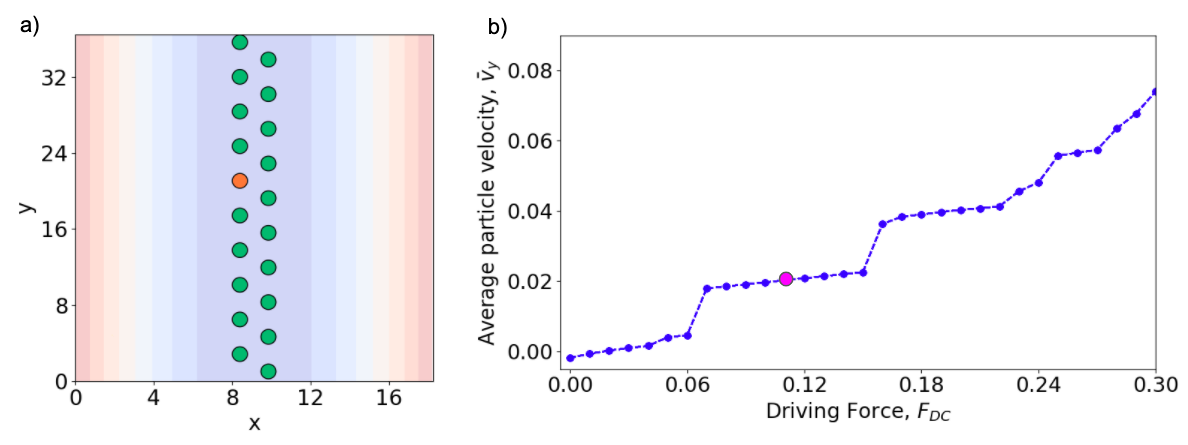
\includegraphics[width=\columnwidth]{twenty}
\caption{\textbf{(a)} A single particle (colored orange - mark in some manner for non-color views) is driven with a constant amplitude $F^{ac}$ and frequency $\omega$ through 19 neighboring particles (colored green - mark differently) confined by a quasi one-dimensional channel. The landscape is colored as in Fig.~\ref{fig1}(a). \textbf{(b)} Average $\langle {v}_{y} \rangle $ versus $F^{dc}$, where $\langle {v}_{y} \rangle$ is the average particle velocity of the driven particle in the y-direction.}
\label{fig:2}
\end{figure}
\end{center}

\section{Kinked system}
\label{sec:kink}	% You can label sections for reference
We confine $N$ particles to $N-1$ troughs to create a
local high density region.
$F^{dc}/F^{ac} = 1$ [CHECK!]
